% ============================================================================
% ch1-introduction.tex — Chapter I: Introduction
% Enriched from working paper part1_intro — all structural content restored
% ============================================================================
\chapterpage{Chapter\kern0.25em I}{Introduction}{images/IM1.jpeg}
\thispagestyle{chapterstart}

\noindent\textit{Data centers are the physical infrastructure of the digital economy---and the only major asset class whose climate exposure has never been financially quantified.}

\vspace{4mm}

\subsection*{When Digital Measures Its Own Risk}
\greensep

\begin{twocolbody}

\noindent In January 2026, a winter storm paralyzed Virginia's data center alley---home to the world's largest concentration of digital infrastructure. Wholesale electricity prices surged from \$200 to \$1{,}800 per MWh overnight \citep{cnbc2026storm}. The PJM\footnote{PJM Interconnection: the regional transmission organization coordinating wholesale electricity in 13 US states and the District of Columbia.} grid approached 147~GW of demand, shattering its previous winter record \citep{pjminsidelines2026}. The Department of Energy issued emergency orders requiring data centers to prepare backup generation \citep{bloomberg2026storm}.

This was not an isolated event. In the same winter, Storm \'{E}owyn knocked out power to over one million customers across Ireland and the United Kingdom, disrupting pan-European cloud workloads \citep{gallagherre2026}. Months earlier, Typhoon Yagi flooded Guangdong province---one of Asia's densest concentrations of digital infrastructure---causing cascading grid failures that took 72~hours to resolve \citep{gallagherre2026}. In the Gulf, temperatures exceeding 50$^\circ$ C pushed cooling systems to their design limits. Each episode exposes a different failure mode---flooding, fuel gelling, cooling exceedance, cascading grid collapse. The common denominator is financial: physical climate hazards now impose direct costs on the infrastructure that supports the digital economy \citep{forzieri2016}.

These are not marginal assets. Data centers are capital-intensive facilities with 15--25~year operational horizons, whose performance depends on energy systems, physical site conditions, and insurance markets---all of which climate change is repricing simultaneously. Governments designate them as critical infrastructure. Capital markets direct trillions toward them. Between 40\% and 60\% of 2035 global capacity will be built in the next five years \citep{iea2025energyai}. Once commissioned, these facilities cannot relocate. Every siting decision made today embeds a quarter-century bet on climate trajectories.

And yet: the sector that hosts the computational infrastructure used for climate projections, that stores the data underpinning TCFD\footnote{Task Force on Climate-related Financial Disclosures.} and CSRD\footnote{Corporate Sustainability Reporting Directive (EU).} disclosures, that prices risk for every other industry---cannot price its own. No valuation framework quantifies how much climate risk a data center carries. No disclosure regime requires the number. No insurance product is calibrated to it. The risk is not unrecognized. It is unpriced.

\end{twocolbody}

\newpage
\subsection*{The Infrastructure at Stake}
\greensep

\begin{twocolbody}

\noindent Data centers have transitioned from commercial real estate to strategic national infrastructure. The scale of capital committed to this transition has no precedent in the sector's history.

\subsubsection*{Compute as strategic infrastructure}

In June 2025, the United States designated hyperscale data centers as Critical Digital Infrastructure---enabling expedited permitting and eligibility for federal risk-sharing programs \citep{thedatascientist2025}. Industry estimates place global economic activity directly dependent on data center operations at \$8.75~trillion by 2027 \citep{equinix2025}---a figure difficult to verify independently, but whose order of magnitude is consistent with the sector's role as transactional backbone of the digital economy. Private investment in US data centers reached record highs in 2024, with Amazon, Microsoft, and Google committing approximately \$210~billion in AI-related capital expenditure \citep{deloitte2025, allianz2025}. Morgan Stanley projects nearly \$3~trillion in global data center spending by 2029; McKinsey estimates cumulative outlays approaching \$7~trillion by 2030 \citep{allianz2025}.

Geopolitical competition reinforces the shift: at the February 2025 AI Action Summit, the EU announced InvestAI, a EUR~200~billion initiative \citep{spglobal2025}. China operates at comparable scale through state-backed programs, with over 25~GW concentrated in the Yangtze Delta, Pearl River Delta, and Beijing-Tianjin corridor. China's ``East Data West Compute'' initiative is redistributing capacity toward western provinces---a strategy that reduces latency costs but increases exposure to seismic and water-stress hazards in regions with less resilient grid infrastructure. The Gulf states deploy sovereign AI infrastructure in regions where ambient temperatures already exceed cooling design thresholds.

\subsubsection*{A decade of documented failures}

The vulnerability of digital infrastructure to physical climate hazards is documented across four distinct failure modes---each mapping onto the economic channels quantified in Chapter~II.

Flooding strikes foundations. Hurricane Sandy (2012) submerged Manhattan basement generators under five feet of water \citep{dcd2012sandy}. Hurricane Harvey (2017) tested Houston facilities at design limits with over 40~inches of rainfall \citep{trgdc2024harvey}. In 2024, severe flooding across Bangladesh and Myanmar disrupted submarine cable landing stations serving regional cloud infrastructure.

Power and grid failure operates differently. Winter Storm Uri (2021) drove temperatures 30--40$^\circ$ F below seasonal norms, causing generator fuel to gel, batteries to fail, and cooling systems to malfunction simultaneously. NERC\footnote{North American Electric Reliability Corporation.} concluded that the ERCOT\footnote{Electric Reliability Council of Texas: the independent system operator managing 90\% of Texas's electric load.} grid came within minutes of uncontrolled cascade failure \citep{datacenterknowledge2021, nerc2025}. The January 2026 Virginia storm confirmed the pattern: wholesale electricity spiked ninefold overnight while the grid approached 147~GW of peak demand.\footnote{The structural dimension of grid stress is visible in PJM's capacity auction for the 2025--2026 delivery year, which cleared at \$269 per MW-day---an 833\% increase from the prior year---with data center load accounting for \$6.5~billion of \$16.4~billion in total capacity costs \citep{utilitydive2026pjm, ieefa2025pjm}.}

Cooling failure is subtler but no less consequential. The July 2022 UK heatwave pushed ambient temperatures above 40$^\circ$ C for the first time in recorded history; Google's London data center and Oracle's UK facility reported outages---not because equipment failed, but because ambient conditions exceeded the thermal envelope within which mechanical cooling was designed to operate \citep{datacenterknowledge2021}. A December 2025 analysis found that nearly 7{,}000 of the world's 8{,}808 operational data centers now sit outside optimal temperature ranges for cooling efficiency \citep{restofworld2025}.\footnote{The 8{,}808 figure is from \citealt{restofworld2025}; this paper's database covers 8{,}572 facilities assembled from a distinct source set.}

Supply chain disruption completes the picture. Typhoon Yagi's flooding of Guangdong province caused cascading grid failures across one of Asia's densest concentrations of digital infrastructure. The 2024 Atlantic hurricane season produced Helene (\$30--47~billion in losses) and Milton (3~million customers without power) in rapid succession \citep{hexatronic2025storms}. The Uptime Institute's 2024 Annual Outage Analysis confirmed that extreme weather was an increasing driver of serious outages industry-wide \citep{techtarget2024}.

These episodes share a structural feature: data centers do not fail in isolation. They fail with grids, supply chains, and cooling systems. NERC warned that data center load growth ``is contributing to continued risk of supply shortfalls'' during extreme weather \citep{nerc2025}; Texas enacted legislation authorizing grid operators to curtail power to data centers during emergencies \citep{spokesman2025}. Global data center electricity consumption reached approximately 450~TWh in 2024, growing at nearly 20\% annually, with preliminary forecasts suggesting over 50~GW of peak capacity in PJM alone by 2030 \citep{iea2025energyai, nrdc2025datacenters}. At this scale, the interaction between demand growth and climate hazards is a permanent feature of the sector's operating environment.

\subsubsection*{Insurance retreat and the protection gap}

Physical hazards damage assets. The investment problem arises from how risk is priced, absorbed, or refused by insurance markets. The global insurance protection gap stood at 56\% in 2025: of \$296~billion in economic losses, \$167~billion went uninsured---a gap growing at 6--10\% annually in real terms \citep{gallagherre2026, swissre2025sigma}. In the EU, only 20\% of natural catastrophe losses are covered \citep{ecb_eiopa2024}. In China, penetration remains below 15\%.

When insurance retreats, asset values follow. Evidence from the US residential market documents declines of 12--48\% in property values following coverage non-renewal \citep{wwf2025}. More than 1.9~million home insurance policies have been non-renewed in the United States since 2018. For data centers, placement programs already exceed \$1~billion, with mega-campuses seeking up to \$3~billion syndicated across multiple insurers \citep{allianz2025}. XDI\footnote{Cross Dependency Initiative: a climate physical risk analytics firm that models asset-level structural damage across eight hazard types.} projects that global insurance premiums for the sector could triple by mid-century \citep{xdi2025}.

When private insurance retreats, governments absorb part of the residual risk. The United States spent approximately \$1~trillion on disaster recovery and climate-related needs in the twelve months to May 2025 \citep{wwf2025}. France has raised catastrophe premium surcharges from 12\% to 20\%, with reinsurer CCR anticipating a 40\% rise in claims by 2050 \citep{hoganlovells2025}.

\subsubsection*{The design window}

Between 40\% and 60\% of 2035 global data center capacity will be built in the next five years \citep{iea2025energyai}. Once commissioned, these facilities cannot relocate. The siting decisions made in this window will embed a quarter-century of climate exposure---or a quarter-century of climate resilience.

The economics of that choice are asymmetric. In the United States, every dollar invested in climate resilience avoids up to \$13 in losses; in the United Kingdom, each GBP~1 spent on flood risk management avoids GBP~8 in damages \citep{wwf2025}. These are among the highest benefit-cost ratios in infrastructure economics. Yet current frameworks for data center siting optimize for power availability, fiber connectivity, and near-term costs. The global project pipeline concentrates investment in markets selected for land access and energy cost rather than climate resilience.

The bottlenecks already identified---grid connection timelines, transformer supply chains with 18--36 month lead times, cooling water availability---are the vectors through which climate hazards translate into financial risk. Every year of delayed adaptation narrows the design window and raises the retrofit cost. The window has not yet closed.

\end{twocolbody}

\vspace{2mm}
\exhibitcaption{1}{Four converging phenomena reshaping data center risk.}

\begin{center}
\datatablesetup
\begin{tabularx}{\textwidth}{>{\raggedright\arraybackslash}p{3.2cm} >{\raggedright\arraybackslash}X >{\raggedright\arraybackslash}p{3cm} >{\raggedright\arraybackslash}p{2.8cm}}
\toprule
\datatableheader
\thd{Phenomenon} & \thd{Evidence} & \thd{Scale} & \thd{Geographic scope} \\
\midrule
\textbf{1. Compute as strategic infrastructure} & Critical infrastructure designations; sovereign AI programs; hyperscaler capex & \$3--7T cumulative investment by 2030 & US, EU, China, Gulf, India, Brazil \\
\textbf{2. Climate hazards disrupt operations} & Sandy, Uri, UK heatwave, Zhengzhou, Typhoon Yagi, Jan.\ 2026 storm & 12+ major events since 2012 & All major DC markets \\
\textbf{3. Insurance retreat} & Protection gap growing 6--10\%/yr; coverage withdrawal; premium escalation & \$167B uninsured in 2025 (56\% gap) & US, EU, Asia, Middle East \\
\textbf{4. Design window closing} & 40--60\% of 2035 capacity built in next 5~yrs; 15--25yr asset horizons & 2$\times$+ installed capacity in pipeline & Global \\
\bottomrule
\end{tabularx}
\datatableclear
\end{center}

% --- Exhibit 2: The scissors — capital IN vs protection OUT ---
\vspace{4mm}
\exhibitcaption{2}{The scissors: capital flowing into data centers accelerates while insurance protection retreats.}

\begin{center}
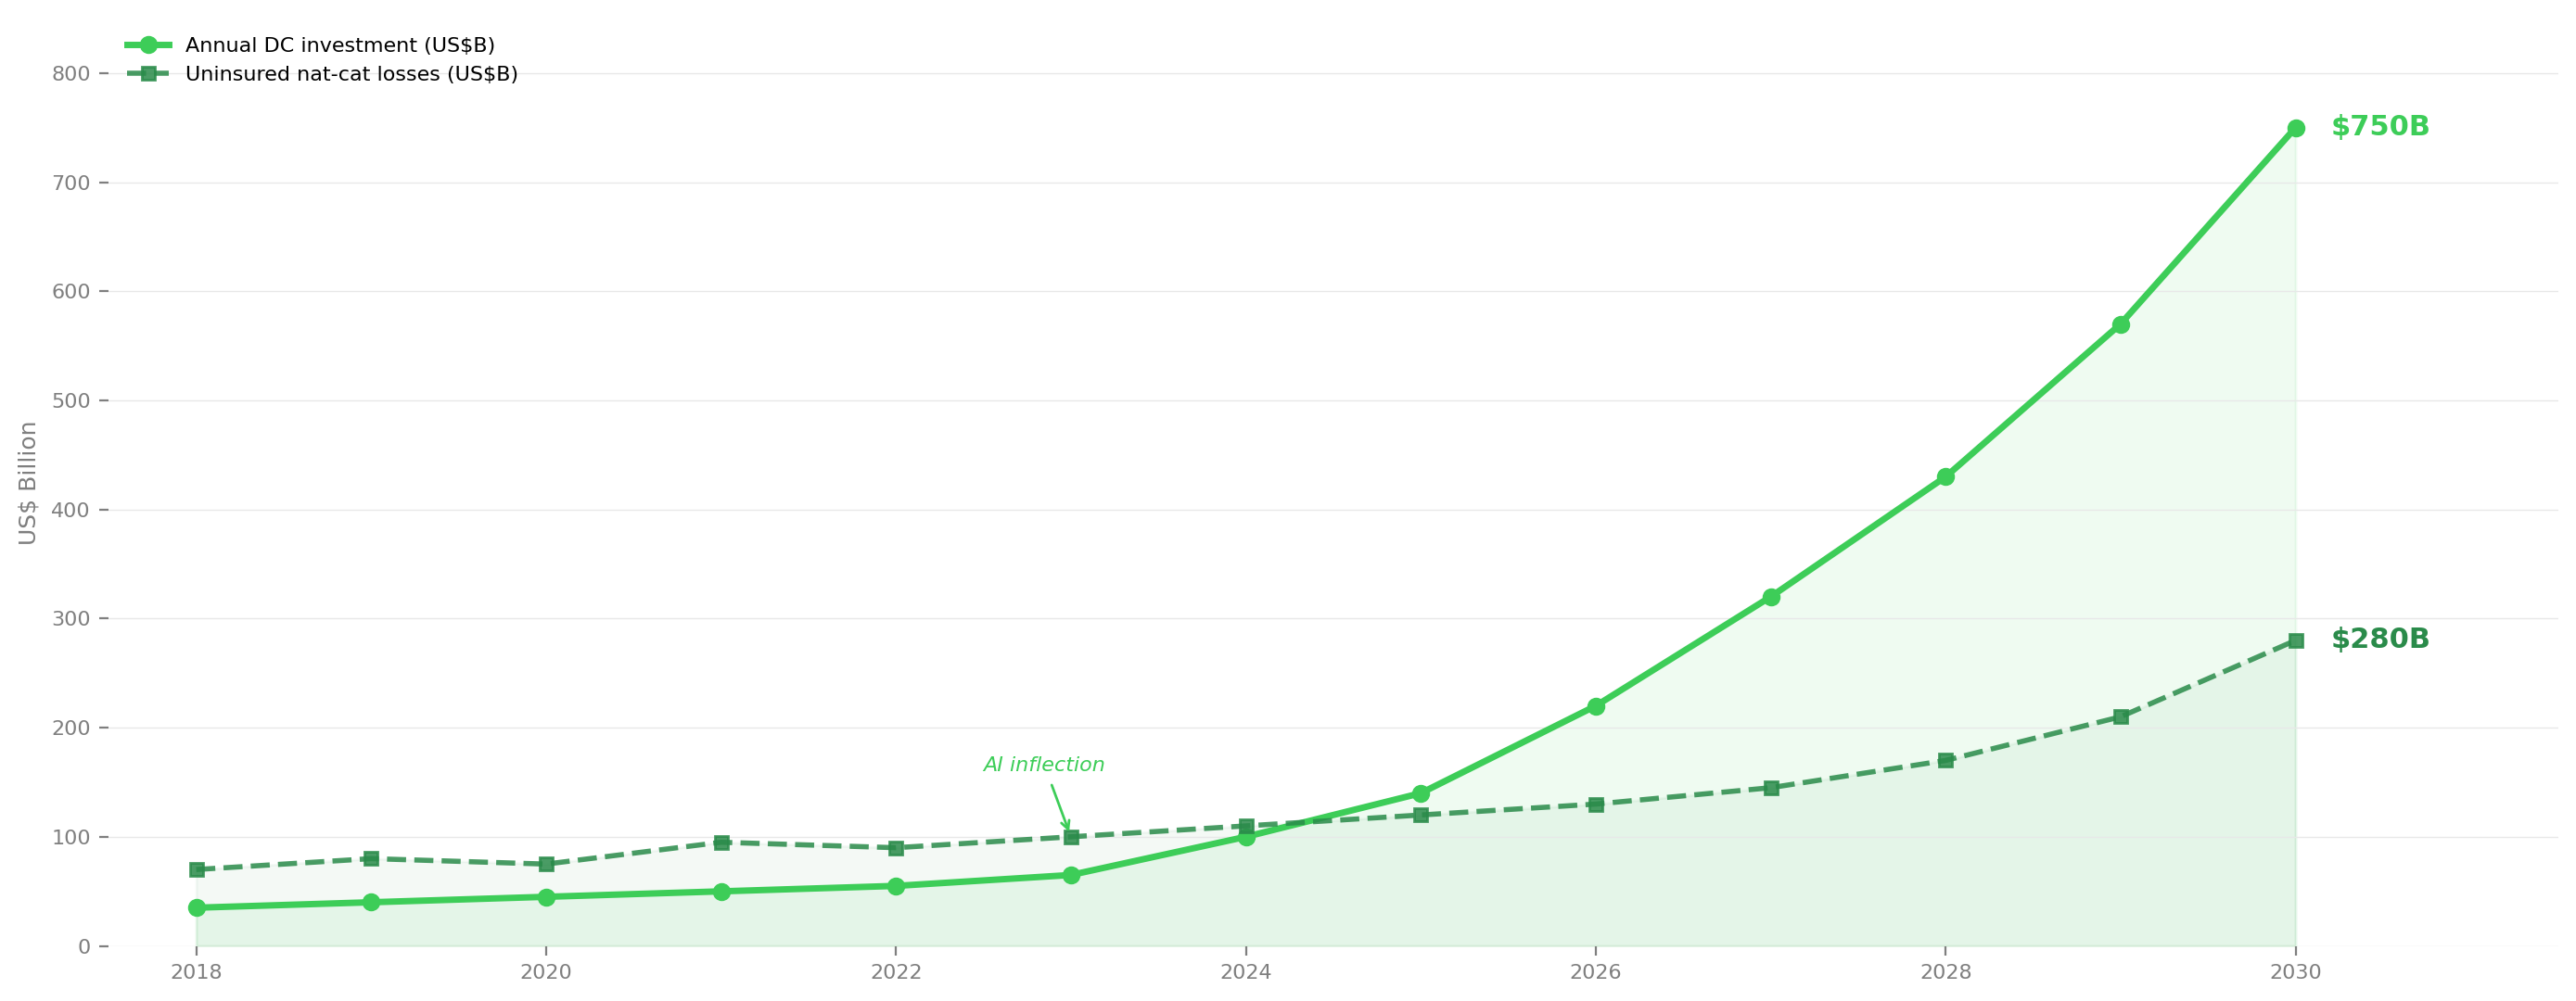
\includegraphics[width=\textwidth]{images/exhibit-scissors.png}
\end{center}
\exhibitsource{Investment data: IEA (2025), McKinsey, Morgan Stanley estimates. Protection gap: Gallagher Re (2026), Swiss Re Sigma. Projections beyond 2025 are indicative.}


\subsection*{The Missing Measurement}
\greensep

\begin{twocolbody}

\noindent These converging pressures raise a direct question: how much climate risk does the global data center sector actually carry? No existing analysis answers it.

\subsubsection*{Academic literature}

Academic research quantifying climate risk for data centers is sparse. A systematic review identified only one sustained program directly addressing the topic---the work of \citet{pasupuleti2022, pasupuleti2024, pasupuleti2025}---compared to hundreds of studies for analogous infrastructure sectors \citep{forzieri2016, dawson2018, oughton2023, luo2023}. This program establishes foundations for flood-aware site selection but does not attempt portfolio-level assessment, does not cover the full range of risk channels, and does not address the AI-era pipeline.

Quantitative frameworks for integrating climate risk into infrastructure valuation exist for energy and transport \citep{in2020, in2021, in2022, prime2018, pasha2025}, but none has been developed or validated for data center assets. The specific vulnerabilities---cooling system dependencies on ambient temperature, power quality requirements, IT equipment sensitivity, and the asymmetric revenue impact of service interruptions relative to physical damage---remain unmodeled. On supply chain propagation, only conceptual treatments exist \citep{koks2022}; no quantitative model links upstream hazards to data center exposure. Compound hazards combining extreme heat, grid stress, and water scarcity remain unaddressed \citep{karagiannakis2024}.

\subsubsection*{Practitioner analyses}

On the practitioner side, three analyses provide the most comprehensive treatments. XDI's 2025 report \citep{xdi2025} covers 8{,}868 facilities across eight hazards with engineering vulnerability functions; major hubs including New Jersey, Hamburg, Shanghai, Tokyo, and Bangkok rank among the top 20 most climate-exposed locations by 2050 \citep{xdi2025, dcd2025}. Its strength is physical engineering precision and coverage of the installed base. By design, it excludes extreme heat---the dominant economic channel for facilities where cooling accounts for 30--50\% of operating costs---and omits transition risk entirely. The report provides a physical hazard map; the translation into financial valuation and the extension to future infrastructure remain open.

The WEF, drawing on S\&P data, produced the first sector-aggregate financial projection: \$3.3~trillion in cumulative climate costs by 2055 \citep{wef2025}. This estimate established financial materiality at board level but operates without facility-level breakdowns or channel decomposition. The underlying methodology has not been published in sufficient detail to enable reproduction.

Verdantix benchmarked 19 physical climate risk vendors across their full capability range \citep{verdantix2024}. Its conclusion is direct: adaptation planning and supply chain risk quantification are the two weakest capabilities across the entire market. The analytical dimensions most relevant to capital allocation are those least developed.

\end{twocolbody}

\vspace{2mm}
\exhibitcaption{3}{Academic literature coverage of climate risk dimensions for data centers.}

\begin{center}
\datatablesetup
\begin{tabularx}{\textwidth}{>{\raggedright\arraybackslash}p{3.2cm} >{\raggedright\arraybackslash}p{4.5cm} >{\raggedright\arraybackslash}X}
\toprule
\datatableheader
\thd{Dimension} & \thd{Coverage} & \thd{Key Gap} \\
\midrule
Physical risk quantification & 3 DC studies \citep{pasupuleti2022, pasupuleti2024, pasupuleti2025}; analogous sectors \citep{forzieri2016, dawson2018, oughton2023} & No sector-wide assessment; cooling and grid interdependencies unmodeled \\
Insurance \& insurability & 1 study, energy focus \citep{kerkhofs2025} & No DC-specific analysis; protection gaps undocumented \\
Valuation frameworks & Multiple for energy/transport \citep{in2020, in2021, in2022} & None developed or validated for data centers \\
Supply chain propagation & Conceptual only \citep{koks2022} & No quantitative models linking upstream hazards to DC exposure \\
Compound hazards & Limited \citep{karagiannakis2024} & Heat + drought + grid stress scenarios unmodeled \\
\bottomrule
\end{tabularx}
\datatableclear
\end{center}

\vspace{4mm}
\exhibitcaption{4}{Analytical scope: existing frameworks versus this paper.}

\begin{center}
\datatablesetup
\begin{tabularx}{\textwidth}{>{\raggedright\arraybackslash}p{3.3cm} >{\centering\arraybackslash}p{1.3cm} >{\centering\arraybackslash}p{1.3cm} >{\centering\arraybackslash}p{1.3cm} >{\centering\arraybackslash}p{1.3cm} >{\raggedright\arraybackslash}X}
\toprule
\datatableheader
& \thd{XDI} & \thd{Pasupuleti} & \thd{WEF/S\&P} & \thd{Verdantix} & \thd{This paper} \\
& \thd{\tiny 2025} & \thd{\tiny et al.} & \thd{\tiny 2025} & \thd{\tiny 2024} & \thd{\tiny SE Research} \\
\midrule
Data Center installed base    & 8,868       & ---         & ---        & ---    & \textbf{8,572} \\
AI pipeline (prospective)        & ---         & ---         & ---        & ---    & \textbf{615--2,939} \\
Investment-grade valuation       & Partial     & Partial     & Partial    & ---    & \textbf{ClimVaR \% EV} \\
Thermal / cooling risk           & ---         & ---         & Partial    & ---    & \textbf{$\gamma$ channel} \\
Transition risk (carbon)         & ---         & ---         & ---        & ---    & \textbf{CC$^{1,2,3}$ + PPA} \\
Channel attribution              & ---         & ---         & ---        & ---    & \textbf{Shapley} \\
Supply chain propagation         & ---         & ---         & ---        & Gap ID & \textbf{Leontief I-O} \\
Scenario architecture            & RCP~8.5     & Partial     & High only  & ---    & \textbf{RCP $\times$ NGFS} \\
Adaptation cost-benefit          & 1 archetype & Site only   & ---        & Gap ID & \textbf{3 pathways} \\
\bottomrule
\end{tabularx}
\datatableclear
\end{center}
\exhibitsource{Full = explicit methodology and sector-wide application; Partial = aggregate or single-site only; --- = not addressed. Gap ID = gap identified but not quantified.}

\begin{twocolbody}

\subsubsection*{Three structural gaps}

Three gaps explain why climate risk remains unpriced. First, existing analyses measure physical hazard intensity or replacement cost---not enterprise value loss, the metric that governs capital allocation, TCFD disclosure, and insurance underwriting. Second, all existing analyses characterize the installed base; none models the prospective AI-era pipeline that represents over 80\% of projected capacity additions. Third, no framework decomposes aggregate risk into actionable economic channels. Without knowing whether a facility's exposure is driven by cooling costs, carbon pricing, physical damage, or supply chain disruption, adaptation budgets cannot be allocated with analytical rigor. Verdantix documents this gap across all 19 vendors it benchmarks; none closes it.

\end{twocolbody}

% ========================================================================
\newpage
\subsection*{What This Paper Does}
\greensep

\begin{twocolbody}

\noindent This paper addresses all three gaps. It asks: \textit{What is the Climate Value at Risk for global data center infrastructure, how does it vary across locations and scenarios, and which adaptation strategies generate positive risk-adjusted returns?}

It makes four contributions. The ClimVaR methodology \citep{epelbaum2025} is adapted to data center infrastructure, embedding physical and transition risks into discounted cash flow analysis through five sector-specific channels: cooling stress, carbon pricing, business interruption, physical damage, and heat productivity loss. Shapley decomposition \citep{shapley1953} attributes each channel's contribution to specific hazards; Leontief input-output analysis \citep{miller2009inputoutput} propagates business interruption through upstream supply chains. Neither tool has previously been applied to this sector. The geocoded database covers 8{,}572 installed facilities and up to 2{,}939 prospective AI-era facilities under three growth scenarios. The scenario architecture crosses warming pathways, transition policies, AI growth trajectories, and adaptation strategies to identify which interventions generate positive returns under which conditions. The adaptation business case is then quantified: proactive strategies reduce aggregate ClimVaR by 30--39\% with positive net present value under every scenario tested---and confirms that all ten do.

\vspace{3mm}

\noindent The valuation framework and the data it requires are the subject of Chapter~II. Chapter~III applies this framework to four questions in sequence: how much risk the sector carries, where it concentrates, how the AI build-out alters the profile, and whether adaptation generates positive returns. The answers are not reassuring on the first three counts. They are on the fourth.

\end{twocolbody}